% Figura Anexo II: el estado estacionario: el capital se acumula hasta que su rendimiento neto iguala la impaciencia
\documentclass[tikz,border=3pt]{standalone}
\usepackage[T1]{fontenc}
\usepackage[utf8]{inputenc}
\usepackage{amsmath}
\usetikzlibrary{arrows.meta,calc,positioning}
\begin{document}
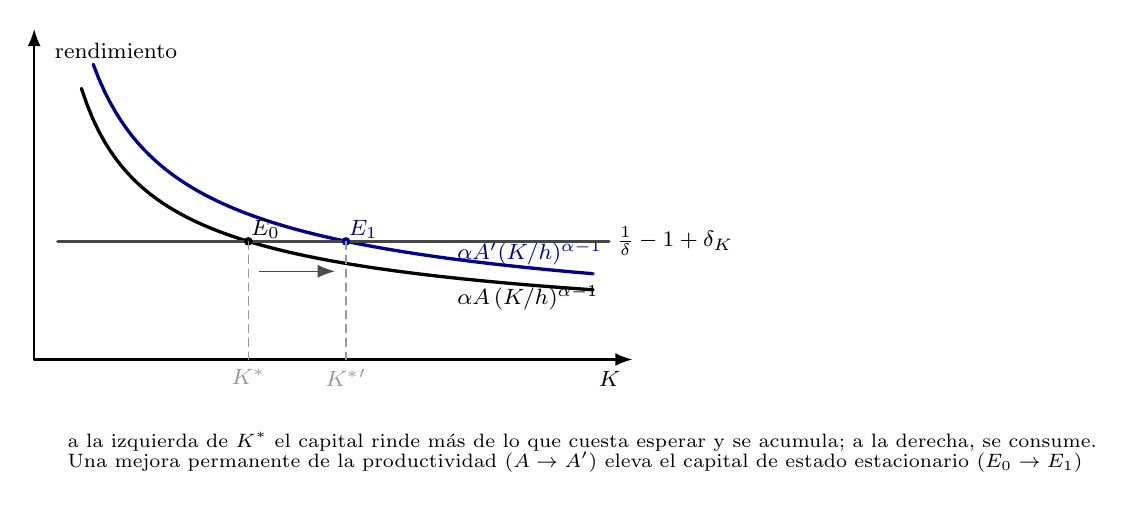
\begin{tikzpicture}[>={Latex[length=2.2mm]}, line cap=round, font=\footnotesize,
  eje/.style={->, thick},
  curva/.style={very thick},
  nueva/.style={very thick, blue!55!black},
  guia/.style={densely dashed, gray!80},
  pto/.style={circle, fill=black, inner sep=1.1pt}]
  \draw[eje] (0,0) -- (7.6,0) node[below left=1pt]{$K$};
  \draw[eje] (0,0) -- (0,4.2) node[below right=2pt]{\;rendimiento};
  \draw[curva, domain=0.6:7.1, samples=90] plot (\x,{2.6*\x^(-0.55)});
  \node[anchor=west] at (5.25,0.78) {$\alpha A\,(K/h)^{\alpha-1}$};
  \draw[nueva, domain=0.75:7.1, samples=90] plot (\x,{3.2*\x^(-0.55)});
  \node[anchor=west, blue!55!black] at (5.25,1.35) {$\alpha A'(K/h)^{\alpha-1}$};
  \draw[curva, gray!55!black] (0.3,1.5) -- (7.3,1.5) node[right=-1pt, black]{$\tfrac{1}{\delta}-1+\delta_K$};
  \node[pto] (E0) at (2.72,1.5) {};
  \node[above right=-2pt of E0, inner sep=1pt] {$E_0$};
  \node[pto, fill=blue!55!black] (E1) at (3.96,1.5) {};
  \node[above right=-2pt of E1, inner sep=1pt, blue!55!black] {$E_1$};
  \draw[guia] (2.72,1.5) -- (2.72,0) node[below]{$K^{*}$};
  \draw[guia] (3.96,1.5) -- (3.96,0) node[below]{$K^{*}{}'$};
  \draw[->, gray!60!black, shorten >=4pt, shorten <=4pt] (2.72,1.12) -- (3.96,1.12);
  \node[align=left, anchor=north west] at (0.3,-0.8) {\scriptsize a la izquierda de $K^{*}$ el capital rinde más de lo que cuesta esperar y se acumula; a la derecha, se consume.\\[-2pt]\scriptsize Una mejora permanente de la productividad ($A\to A'$) eleva el capital de estado estacionario ($E_0\to E_1$)};
\end{tikzpicture}
\end{document}
